\documentclass{beamer}
\usetheme{Warsaw}
\usepackage{graphicx}
\usepackage[czech]{babel}
\usepackage[utf8]{inputenc}
\usepackage{times}
\usepackage{hyperref}
\usepackage[czech,ruled,linesnumbered]{algorithm2e}

\setbeamertemplate{footline}[frame number]

\title{Růst domácností a jeho dopad na energetiku}
\author{Smirnov Nikita}
\date{\today}

\begin{document}

\begin{frame}
    \titlepage
\end{frame}

\section{Úvod}
\subsection{Motivace}
\begin{frame}{Počet domácností v ČR i ve světě dlouhodobě roste. Co to znamená pro spotřebu energie a jaké výzvy to přináší do budoucna?}
    \only<1>{
        \begin{block}{Pozorování}
            I přes to, že růst světové populace se zpomaluje díky moderním technologiím a vzdělání, 
            \textbf{průměrný počet osob na domácnost klesá}.  
            Výsledkem je, že \textbf{počet domácností nadále rychle roste}.
        \end{block}
    }
    \only<2>{
        \begin{figure}[ht]
            \centering
            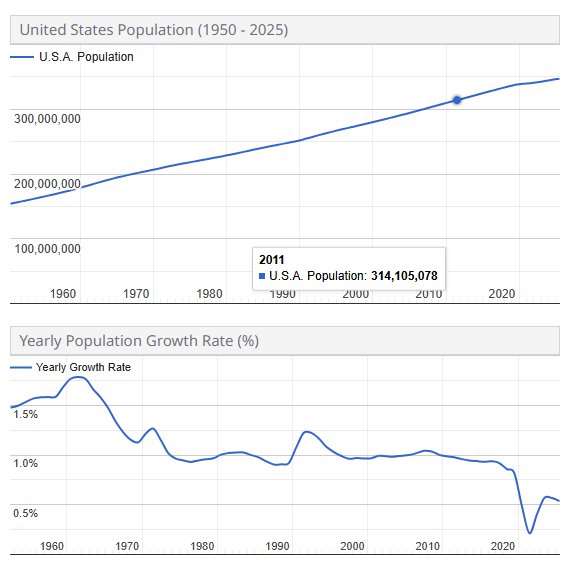
\includegraphics[width=0.45\textwidth]{population.png}
            \hfill
            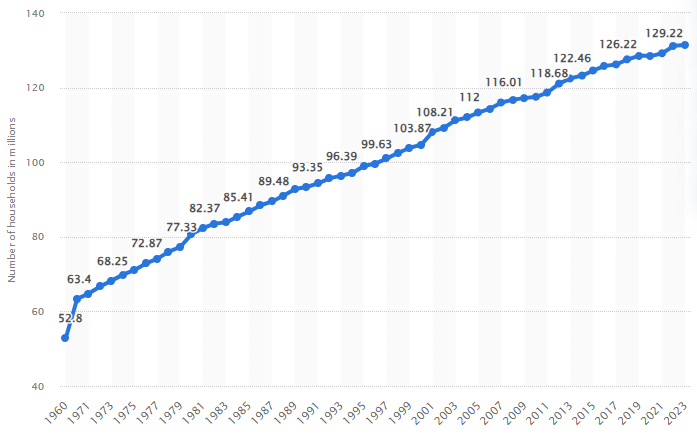
\includegraphics[width=0.45\textwidth]{households.png}
            \caption{Růst populace (vlevo) a počet domácností (vpravo)}
        \end{figure}
    }
\end{frame}

\subsection{Cíl projektu}
\begin{frame}{Více domácností = vyšší nároky na energetickou síť?}
    \only<1>{
        \begin{block}{Pozorování}
            V posledních 30 letech \textbf{počet domácností roste rychleji než počet obyvatel}.
            
            \centering
            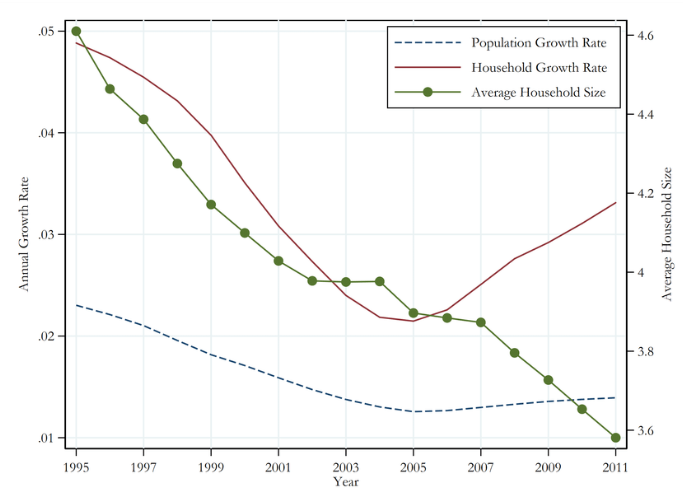
\includegraphics[width=0.7\textwidth]{householdVSpopulation.png}
        \end{block}
    }

    \only<2>{
        \begin{block}{Důsledek}
            Každá domácnost má základní spotřebu:  
            \textit{osvětlení, topení, spotřebiče, elektronika}.

            \centering
            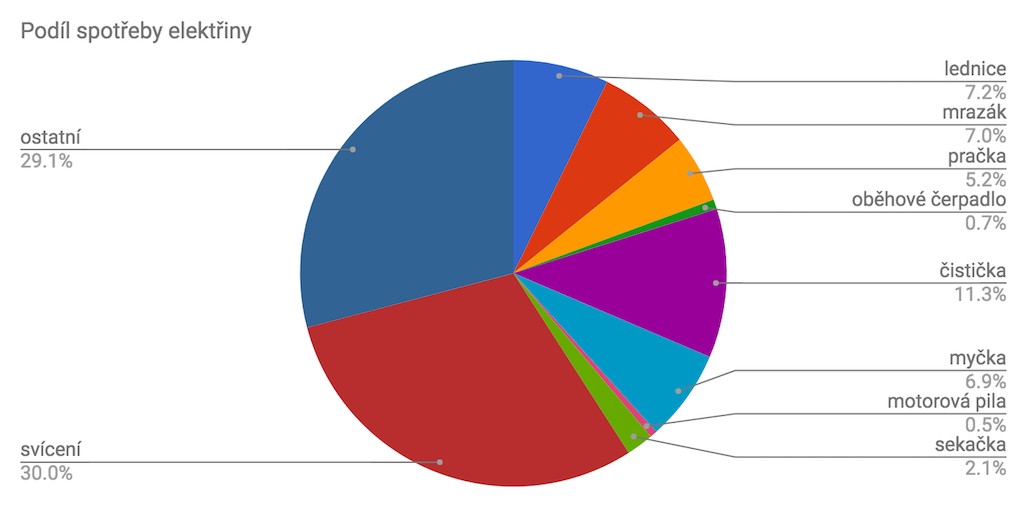
\includegraphics[width=1\textwidth]{podilSpot.png}
        \end{block}
    }

    \only<3>{
        \begin{block}{Problém}
            Rostoucí zatížení sítě → potřeba \textbf{regulace} a \textbf{predikce spotřeby}.

            \centering
            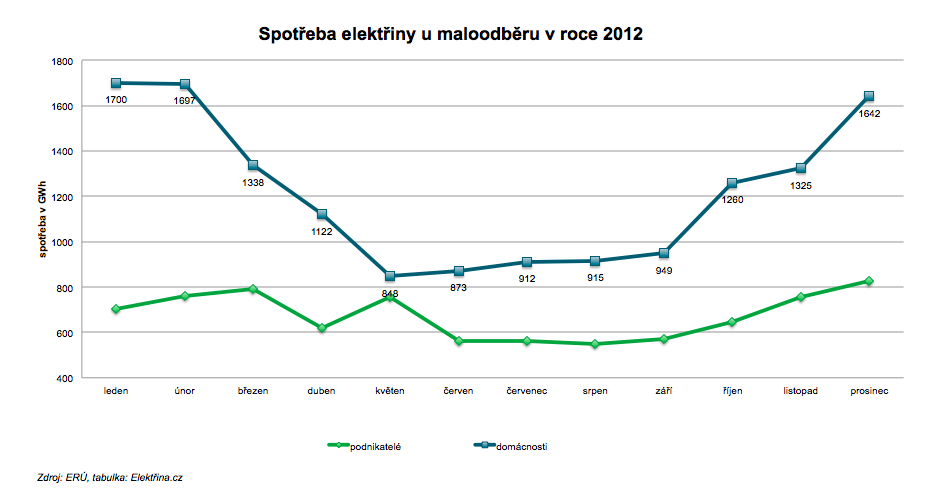
\includegraphics[width=0.9\textwidth]{spotrebaEl.png}
        \end{block}
    }
\end{frame}

\begin{frame}{Cíl projektu}
    Analyzovat vývoj spotřeby a modelovat vliv růstu domácností pomocí \textbf{simulačního nástroje}.
\end{frame}


\section{Simulační model}
\subsection{Vyjádření modelu}
\begin{frame}{Návrh simulačního modelu}
    \begin{block}{Funkce pro výpočet spotřeby energie pro jednu domácnost}
    \[E_h(t) = E_{hprev} \cdot P(t)^{\beta_P} \cdot GDP(t)^{\beta_{GDP}} \cdot Eff(t)^{\beta_{eff}}\]
    kde:
    \begin{itemize}
        \item $E_{hprev}$ - spotřeba energie v předchozím roce.
        \item $P(t)^{\beta_P}$ - cena energie v tomto roce, s ohledem na koeficient elasticity.
        \item $GDP(t)^{\beta_{GDP}}$ - HDP v tomto roce, s ohledem na koeficient elasticity.
        \item $Eff(t)^{\beta_{eff}}$ - energetická účinnost, s ohledem na koeficient elasticity.
        \item $\beta_P, \beta_{GDP}, \beta_{eff}$ - jsou koeficienty elasticity, které popisují, změna každého faktoru ovlivňuje poptávku po energii.
    \end{itemize}
    \end{block}
\end{frame}

\begin{frame}{Návrh simulačního modelu}
    \begin{block}{Funkce pro výpočet počtu domácností}
    \[H(t) = H_{prev} \cdot \bigg(1 + r_{H} \cdot \cfrac{GDP(t)}{GDP_{prev}}\bigg)\]
    kde:
    \begin{itemize}
        \item $H_{prev}$ - počet domácností v předchozím roce.
        \item $r_{H}$ - 0.015, vypočtený standardní procento růstu domácností.
        \item $\cfrac{GDP(t)}{GDP_{prev}}$ - faktor růstu HDP za poslední rok.
    \end{itemize}
    \end{block}
\end{frame}

\begin{frame}{Návrh simulačního modelu}
    \begin{block}{Funkce pro výpočet ceny elektřiny}
    \[P(t) = P_{prev} \cdot e^{\beta \cdot (t-t_{prev})}\]
    kde:
    \begin{itemize}
        \item $P_{prev}$ - cena elektřiny v předchozím roce.
        \item $\beta$ - 0.015, vypočtený faktor růstu ceny pro exponenciální funkci.
    \end{itemize}
    \end{block}
        
    \uncover<2>{
        \begin{block}{Funkce pro výpočet HDP}
        \[GDP(t) = GDP_{prev} \cdot (1 + r_{GDP} \cdot (t-t_{prev}))\]
        kde:
        \begin{itemize}
            \item $GDP_{prev}$ - HDP v předchozím roce.
            \item $\beta$ - 0.025, faktor růstu HDP.
        \end{itemize}
        \end{block}
    }
\end{frame}

\begin{frame}[fragile]{Pseudokód pro simulaci jednoho roku}
\begin{algorithm}[H]
\setcounter{algocf}{0}
\SetKwInOut{Input}{Vstup}
\SetKwInOut{Output}{Výstup}

\only<1> {
    \Input{Seznam dat \texttt{data}, počáteční rok \texttt{startYear}, koncový rok \texttt{endYear}}
    \Output{CSV soubor se simulovanými hodnotami spotřeby energie}

    nastav \texttt{efficiency} na 1.0\;
    nastav \texttt{energyConsumption} na \texttt{BASE\_CONSUMPTION}\;
}

\For{rok \texttt{year} od \texttt{startYear} do \texttt{endYear}}{
    \only<1> {
        \texttt{gdp} $\gets$ \texttt{calculateGDP(data, year)}\;
        \texttt{households} $\gets$ \texttt{calculateHouseholds(data, year, gdp)}\;
        \texttt{energyPrice} $\gets$ \texttt{calculateEnergyPrice(data, year)}\;
    }
    \only<2>{
        \texttt{energyConsumption} $\gets$ \texttt{calculateEnergyConsumptionPerHousehold(...)}\;
        \texttt{totalCons} $\gets$ \texttt{energyConsumption} $\times$ \texttt{households}\;
    zapiš do CSV: \texttt{year, households, gdp, ...}\;
        \texttt{addNewYearData(...)}\;
        \texttt{efficiency} $\gets$ \texttt{efficiency} $\times$ (1.0 $+$ \texttt{EFF\_GROWTH})\;
    výstup na konzoli: rok, domácnosti, GDP, cena, spotřeba\;
    }
}
\caption{Simulace spotřeby – výpočet vstupních veličin}
\end{algorithm}
\end{frame}

\subsection{Validita modelu}
\begin{frame}{Vyhodnocení simulačního modelu}
    Porovnání se skutečnými daty ukazuje, že model dokáže predikovat vývoj spotřeby energie na základě růstu počtu domácností a dalších faktorů, což jej činí vhodným nástrojem pro analýzu a predikci energetických nároků v budoucnosti.
\begin{figure}[H]
\centering
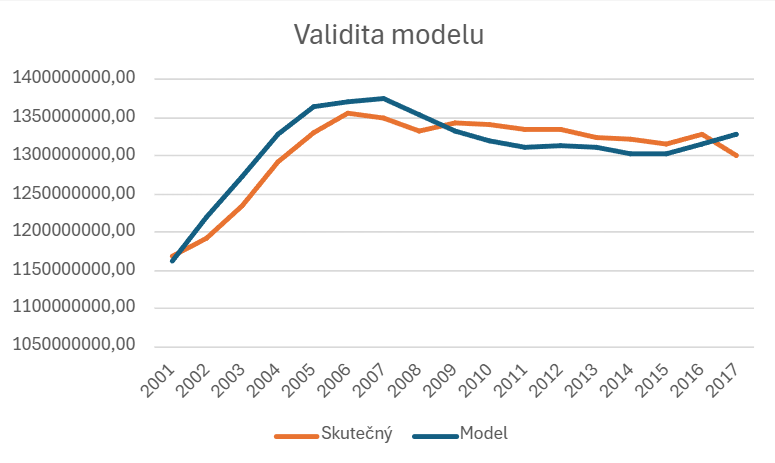
\includegraphics[width=0.8\linewidth]{valid_model_gr.png}
\end{figure}
\end{frame}

\end{document}
